%!tex root = ../main.tex

\section{Algorithm} \label{sec:algorithm}

In this section, we will introduce the basic idea of an essential algorithm that is used in the actual implementation discussed in section \ref{sec:implementation}.
The algorithm's purpose is to find a proof that a given LCL problem $\Pi$ is impossible to solve in PN model.
Here we specifically allow PN networks to have multiple connections.
Later in the Section \ref{sec:algorithm:theorems:a} we show that the unsolvability of a problem $\Pi$ in PN networks (with multiple connections) implies that it is also impossible to solve $\Pi$ in \emph{simple} PN networks (without multiple connections).
Finally in the Section \ref{sec:algorithm:theorems:b} we show that the unsolvability of $\Pi$ in \emph{simple} PN networks implies that $\Pi$ is not solvable in constant time ($\mathcal{O}(1)$) in the LOCAL model.

%TODO These definitions and theorems might have a better place under section 2 background.
\begin{definition} \label{def:lcl_solvability}
    An LCL problem $\Pi$ is solvable in PN model, if and only if there exists a PN algorithm $A$ that finds a solution for $\Pi$ in all PN networks.
\end{definition}

We can define an alternative version of the Definition \ref{def:lcl_solvability} using contraposition.
\begin{definition} \label{def:lcl_solvability:contrapositive}
An LCL problem $\Pi$ is not solvable in PN model, if and only if there \textbf{does not exist} a PN algorithm $A$ that finds a solution for $\Pi$ in all PN networks.
\end{definition}

The Definitions \ref{def:lcl_solvability} and \ref{def:lcl_solvability:contrapositive} are equivalent. The latter one might be more difficult to understand, but the way it is phrased, easily leads us to the following Theorem:

\begin{theorem} \label{thm:lcl_nonsolvability}
    An LCL problem $\Pi$ is not solvable in PN model, if there exists a PN network $N$ such that no PN algorithm $A$ can solve the $\Pi$ in $N$.
\end{theorem}
\begin{proof}
    Let $\Pi$ be an LCL problem.
    Let $N$ be a PN network such that no PN algorithm $A$ can solve $\Pi$ in $N$.
    Therefore no PN algorithm $A$ can find a solution to $\Pi$ in all PN networks.
    According to the definition \ref{def:lcl_solvability:contrapositive}, this is equivalent with $\Pi$ being unsolvable.
\end{proof}

As the Theorem \ref{thm:lcl_nonsolvability} shows us, to show that a problem $\Pi$ is unsolvable, it is enough to find a counterexample, a PN network $N$ in which the problem $\Pi$ cannot be solved.
To show that, it is enough to find an underlying graph $G$ of $N$ in which the problem $\Pi$ cannot be solved.
Using this fact, we can come up with an algorithm that automatically tries to find an counterexample graph.

\begin{algorithm}[H]
    \caption{Counterexample graph finder algorithm}
    \label{alg:counterexample_finder}
    \begin{algorithmic}[1] % The number tells where the line numbering should start
        \Require $1 \leq n_{low} \leq n_{high}$
        %\Require $\Pi$ is an LCL problem
        \Function{Find}{$n_{low},n_{high}, \Pi$} \Comment{Graph bounds $n_{low}$ and $n_{high}$, LCL problem $\Pi$} \label{alg:counterexample_finder:n_loop}
            \State $d_a \gets \textsc{ActiveDegree}(\Pi)$ \label{alg:counterexample_finder:d_a}
            \State $d_p \gets \textsc{PassiveDegree}(\Pi)$ \label{alg:counterexample_finder:d_p}
            \For{$n\gets n_{low}, n_{high}$} \Comment{Iterate graph sizes from lowest to highest} \label{alg:counterexample_finder:n}
                \State $G_n \gets \textsc{GenerateGraphs}(n, d_a, d_p)$ \label{alg:counterexample_finder:Gn}
                \ForEach{$g \in G_n$} \label{alg:counterexample_finder:g}
                    \If {$\textsc{IsUnsolvable}(\Pi, g)$} \label{alg:counterexample_finder:is_unsolvable}
                        \State \Return $g$ \label{alg:counterexample_finder:return_g}
                    \EndIf
                \EndFor
            \EndFor
            \State \Return \Comment{No counterexample found. Return nothing.} \label{alg:counterexample_finder:return_nothing}
        \EndFunction
    \end{algorithmic}
\end{algorithm}

The Algorithm \ref{alg:counterexample_finder} is designed to find the smallest counterexample graph for an LCL problem $\Pi$.
It starts from graphs of size $n_{low}$ and goes up to graphs of size $n_{high}$.
%TODO define what is a graph's size, in 2. background.
We define $d_a$ and $d_p$ to be the active and passive degree of the problem $\Pi$ respectively (rows \ref{alg:counterexample_finder:d_a} and \ref{alg:counterexample_finder:d_p}).
The variable for the current graph size is called $n$ (row \ref{alg:counterexample_finder:n}).
For each graph size $n$, we generate all possible $(d_a, d_p)$-biregular multigraphs with $\textsc{GenerateGraphs}(n, d_a, d_p)$, and save the graphs into variable $G_n$ (row \ref{alg:counterexample_finder:Gn}).
The reason for generating only these types of graphs comes from our definition of LCL problem from section \ref{sec:lcl_problems}, they are defined specifically for $(b,a)$-biregular (multi)graphs.
%TODO make sure that it defines the LCL problems we are using here (LCL for (b,a)-biregular graphs)
Now, for each graph $g \in G_n$ (row \ref{alg:counterexample_finder:g}) we check if the given problem $\Pi$ is unsolvable using the function $\textsc{IsUnsolvable}(\Pi, g)$ (row \ref{alg:counterexample_finder:is_unsolvable}).
If it is unsolvable, we return the graph as an counterexample (row \ref{alg:counterexample_finder:return_g}).
In the case there are no counterexamples in graphs of size $n_{low}$ to $n_{high}$, the algorithm returns nothing (row \ref{alg:counterexample_finder:return_nothing}).

Up to this moment, we have not discussed about how the function $$\textsc{GenerateGraphs}(n, d_a, d_p)$$ from row \ref{alg:counterexample_finder:Gn} generates the graphs, nor have we discussed about how the function $$\textsc{IsUnsolvable}(\Pi, g)$$ from row \ref{alg:counterexample_finder:is_unsolvable} determines the unsolvability used in the Algorithm \ref{alg:counterexample_finder}.
These functions are implementation specific and in this section we assume that they exist as black boxes.
Later on the section \ref{sec:implementation} we introduce our implementations of these functions.
%First we would like to discuss about the $\textsc{GenerateGraphs}(n)$.
%As we know from the section \ref{}, %TODO refer to LCL section and make sure that it defines the LCL problems we are using here (LCL for (b,a)-biregular graphs).
%the LCL problems used in this thesis are defined for $(b,a)$-biregular graphs.
%Therefore we should not generate \emph{all} graphs but only the graphs of type $(b,a)$-biregular, where the degrees $b$ and $a$ are taken from the LCL problem $\Pi$.



%TODO talk about graphs, why they are actually (b, a)-biregular multigraphs.
%TODO talk about networks and graphs. In the above text they are refered as if they were the same thing.
%TODO Do we need to talk about trees and how these biregular multigraphs relate to them? 'Informally, the idea is to prove negative results for the case in which "we are in the middle of a very large tree, far away from the leaves".'

In the following sections, we will prove that if an LCL problem $\Pi$ is not solvable in PN network $N$ with multiple connections, then it is not solvable in constant time in the LOCAL model.
We have divided the proofs into multiple theorems and grouped them under two different sections, Section \ref{sec:algorithm:theorems:a} and Section \ref{sec:algorithm:theorems:b}.
The dependencies of theorems are shown in the Figure \ref{fig:algorithm:theorem_dependency}.
\footnote{Where should I put these theorems? Do they fit under Section \ref{sec:algorithm}?}

\begin{figure}[H]
    \centering
    % https://tex.stackexchange.com/a/499577
    \begin{tikzpicture}[]
        \node (1) [] {Theorem \ref{thm:lcl_nonsolvability:2}};
        \node (2) [right = of 1] {Theorem \ref{thm:lcl_nonsolvability:3}};
        \node (3) [below = of $(1)!0.5!(2)$] {Theorem \ref{thm:lcl_nonsolvability:4}};
        \node (4) [below = of 3] {Theorem \ref{thm:lcl_nonsolvability:5}};
        %\node (4) [right = of mat2-2-1] {$\deg_G(4)=2$};
        %\node (5) [right = of mat2-3-1] {$\deg_G(5)=2$};
        \draw[<-] (1) edge (3);
        \draw[<-] (2) edge (3);
        \draw[<-] (3) edge (4);
    \end{tikzpicture}
    \caption{A dependency graph of the following theorems.\label{fig:algorithm:theorem_dependency}}
\end{figure}

\subsection{\todo{Theorems A}} \label{sec:algorithm:theorems:a}
In this section we show that if an LCL problem is not solvable in PN networks with multiple connections, then the problem is also not solvable in simple PN networks.
We try to split this into couple of theorems and at the end utilize the shown theorems to show this to be true.

% Pi is nonsolvable in multiple connection PN network N -> Pi is nonsolvable in lift of N
\begin{theorem} \label{thm:lcl_nonsolvability:2}
If an LCL problem $\Pi$ is not solvable in PN network $N$, then it is also not solvable in any PN network $N'$ that is a lift of $N$.
\end{theorem}
\begin{proof}
    Let problem $\Pi$ have no solution in some PN network $N$.
    Then any algorithm $A$ produces a result that is nonvalid solution to $\Pi$ i.e. a local constraint is violated at least at some node $v$.
    Let $\phi: V' \rightarrow V$ be a covering map from $N'=(V', P', p')$ to $N=(V, P, p)$
    Theorem 7.1. \footnote{\todo{should I show the theorem or is this enough?}} from the text book \cite{HirvonenSuomelaDistAlg2020} shows that the nodes of $N'$ will have exactly the same state as their counterparts at $N$ for each time unit $t=0,1,...$.
    Hence if we run algorithm $A$ on both networks $N$ and $N'$, the local constraint violation at some node $v \in N$ also appears in all nodes $v' \in V'$ such that $\phi(v') = v$ i.e. the local constraint violations also appear in the covering network $N'$.
\end{proof}

% Network with multiple connections ----k-lift--->  simple network
\begin{theorem} \label{thm:lcl_nonsolvability:3}
    If there is a PN network $N_2$ with multiple connections with $k$ being the highest count of multiple connections between any two nodes, then there exists a $k$-lift $N_1$ of $N_2$ such that $N_1$ is a simple PN network.
\end{theorem}
\begin{proof}
    Let $N_2=(V_2, P_2, p_2)$ be a PN network with multiple connections.
    Let $\operatorname{mul}(u, v)$ be the number of connections between any nodes $u, v \in V_2$.
    Let $k=\max (\{ m(u, v) | u, v \in V_2\} )$ i.e. the highest count of multiple connections.
    \footnote{\todo{Is the "maximum number of multiple connections" ambiguous? Does it appear as the highest count of parallel connections or as the total number of multiple connections in the network?}}
    Let $\operatorname{M}(x+hk) = x$ for all $x = 1, ..., k$ and $h\in \mathbb{N}$ i.e. $\operatorname{M}$ maps positive integers to positive integers under modulo $k$, for example $\operatorname{M}(1 + hk) = 1$ and $\operatorname{M}(k + hk) = k$.

    Let there be another network $N_1=(V_1, P_1, p_1)$ such that:
    \begin{itemize}
        \item For each $v \in V_2$, there are $k$ clones in $V_1$, namely the nodes $v_1, v_2, ..., v_k \in V_1$.
        Thus the sizes $|V_1|$ and $k|V_2|$ are equal.
        %$V_1 = \{v_x: \forall v \in V_2, \forall x \in \{1, 2, ..., k\}\}$
        \item For each port $(v, i) \in P_2$, we have each port $(v_x, i) \in P_1$ where $x=1, 2, ..., k$.
        %% TODO remove these comments when this has been reviewed.
        %\item For each non-multiple connection $p_2((v, i)) = (u, j)$, we have connections $p_1((v_x, i)) = (u_x, j)$, where $x=1, 2, ..., k$.
        %\item For each multiple connections $p_2((v, i_a)) = (u, j_a)$ where $a = 1, 2, ..., \operatorname{mul}(u, v)$, we have $p_1((v_{x}, i_a)) = (u_{\operatorname{M}(x+a-1)}, j_a)$.
        %Note that the non-multiple connections are just a special case where $a$ is always $1$.

        \item For each connection $p_2((v, i_a)) = (u, j_a)$ where $a = 1, 2, ..., \operatorname{mul}(u, v)$, we have $p_1((v_{x}, i_a)) = (u_{\operatorname{M}(x+a-1)}, j_a)$.
        Note that if $\operatorname{mul}(u, v) = 1$, then $p_1((v_{x}, i_1)) = (u_{\operatorname{M}(x)}, j_1) = (u_{x}, j_1)$.
    \end{itemize}

    Now we show that there is a covering map $\phi: V_1 \rightarrow V_2$.
    Let $\phi(v_x) = v \in V_2$ for each $v_x \in V_1$ where $x=1, 2, ..., k$.
    We will show that $\phi$ is a covering map using the Definition \ref{def:covering_map}:
    \begin{itemize}
        \item By the definition of $\phi$, it is surjective.
        \item For each connection in $N_2$, we have $k$ similiar connections in $N_1$, therefore degrees of each node are preserved.
        %% TODO remove these comments when this has been reviewed.
        %\item For each non-multiple connection $p_1((v_x, i)) = (u_x, j)$, where $x=1, 2, ..., k$, we have $p_2((v, i)) = (u, j)$.
        %From our definition of $\phi$ we can see that the mapping preserves port numbers and connections in non-multiple connections.
        %\item For each multiple connection $p_1((v_{x}, i_a)) = (u_{\operatorname{M}(x+a-1)}, j_a)$ we have
        %\begin{align*}
        %    p_2((\phi(v_{x}), i_a)) &= (\phi(u_{\operatorname{M}(x+a-1)}), j_a)\\
        %    \Leftrightarrow p_2((v, i_a)) &= (u, j_a)
        %\end{align*}
        %Both $(v, i_a)$ and $(u, j_a)$ are in $P_2$ and $p_2((v, i_a)) = (u, j_a)$, therefore for each multiple connection, the port numbers and connections are preserved.
        \item For each connection $p_1((v_{x}, i_a)) = (u_{\operatorname{M}(x+a-1)}, j_a)$ we have
        \begin{align*}
           p_2((\phi(v_{x}), i_a)) &= (\phi(u_{\operatorname{M}(x+a-1)}), j_a)\\
           \Leftrightarrow p_2((v, i_a)) &= (u, j_a)
        \end{align*}
        Both $(v, i_a)$ and $(u, j_a)$ are in $P_2$ and $p_2((v, i_a)) = (u, j_a)$, therefore for each connection, the port numbers and connections are preserved.
    \end{itemize}
    Each condition holds, hence the function $\phi$ is a covering map from $V_1$ to $V_2$
    therefore $N_1$ is a $k$-lift of $N_2$.

    We need to show that $N_1$ is a simple PN network i.e. it does not have multiple edges.
    %As we know, the non-multiple connections in $N_2$ are preserved in $N_1$ therefore we need to only look at the multiple connections of $N_2$ in more detail.
    We know that there are connections $p_1((v_{x}, i_a)) = (u_{\operatorname{M}(x+a-1)}, j_a)$ where $a=1, 2, ..., \operatorname{mul}(\phi(v_{x}),\phi(u_{\operatorname{M}(x+a-1)}))$.
    We see that nodes $u_{\operatorname{M}(x+a-1)}$ are distinct for all $a$ because $1 \leq a \leq \operatorname{mul}(\phi(v_{x}),\phi(u_{\operatorname{M}(x+a-1)})) \leq k$, $1 \leq \operatorname{M}(x+a-1) \leq k$ and
    there are exactly k many "u" nodes in $V_1$, namely nodes $u_1, u_2, ..., u_k \in V_1$.
    Thus for each node $v_x$, all connections from $v_x$ are mapped to distinct nodes, therefore $N_1$ is simple.

    It might not be clear that $N_1$ is connected, thus we show next that this is the case.
    The network $N_2$ is connected by the assumption (Section \ref{sec:underlying_graph}).
    Let u
    \begin{itemize}
        \item Let us look at all connections in $p_1$ and fix $a=1$.
        Then $p_1((v_{x}, i_a)) = (u_{\operatorname{M}(x+a-1)}, j_a)$
        $=p_1((v_{x}, i_1)) = (u_{x}, j_1)$.
        This shows that we can traverse from any node $w_x\in P$ to any other node $w'_x\in P$ only using nodes with subscript $x$.
        \item[$a>1$]:
        There are at least some nodes $u, v \in P_2$ such that $\operatorname{mul}(u,v) = k$, therefore we can traverse from any $u_x \in P_1$ to any $v_y \in P_1$ for any $x, y \in \{1, 2, ..., k\}$.
    \end{itemize}
    Thus $N_1$ is connected.
\end{proof}

%\begin{figure}[H]
% \centering
% \includegraphics[]{example-image-duck}
% \caption{\todo{Illustration of k-lift using Theorem \ref{thm:lcl_nonsolvability:3}}}
% \label{fig:duck2}
%\end{figure}

\begin{figure}[H]
    \subcaptionbox{
      A PN network $N_2$ with multiple connections.
      \label{fig:algorithm:k-lift_proof_simple1:a}
    }%
      [.5\linewidth] {
      \centering
      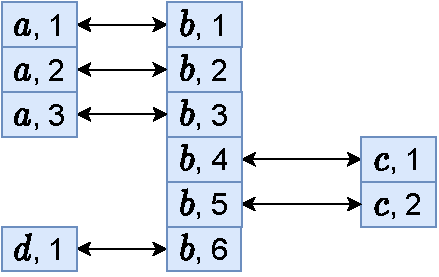
\includegraphics[scale=0.55]{diagrams/algorithm_k-lift_proof_simple_1.pdf}
    }
    \hfill
    \subcaptionbox{
      A simple PN network $N_1$.
      \label{fig:algorithm:k-lift_proof_simple1:b}
    }%
      [.5\linewidth] {
      \centering
      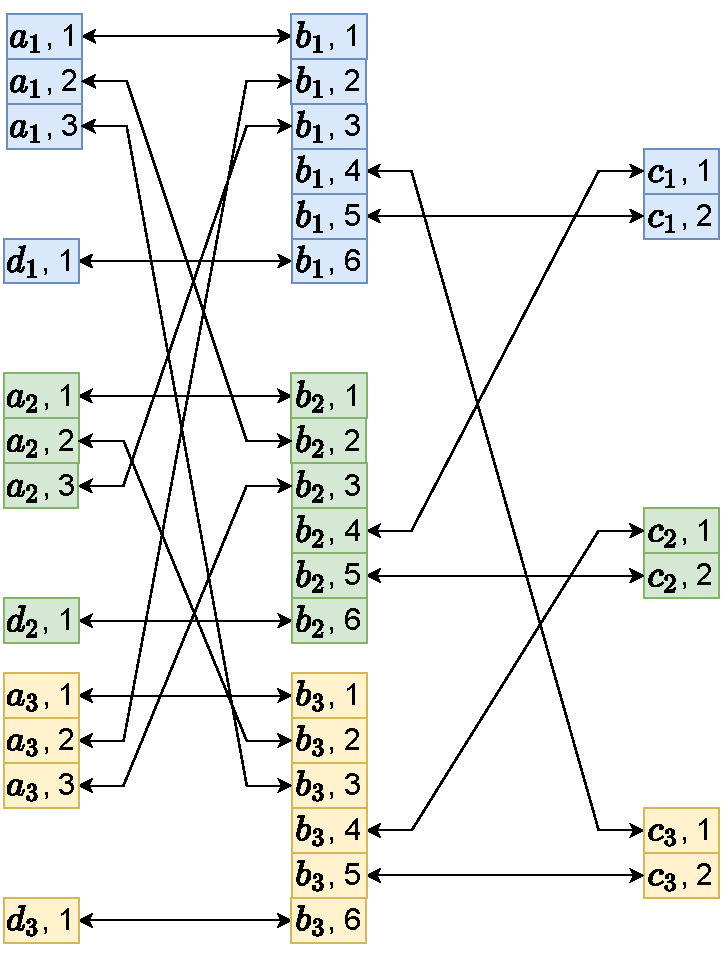
\includegraphics[scale=0.55]{diagrams/algorithm_k-lift_proof_simple_2.pdf}
    }
    \caption{The network $N_1$ is a 3-lift of the network $N_2$.
    }
    \label{fig:algorithm:k-lift_proof_simple1}
  \end{figure}


%% This is more like an instruction on how to build the network, not a proof or is it?

    % Let $N=(V, P, p)$ be a PN network with multiple connections.
    % Let $m(u, v)$ be the number of connections between any nodes $u, v \in V$.
    % Let $k=\max {m(u, v) | u, v \in V}$ i.e. the maximum number of multiple connections.
    % \footnote{\todo{Is the "maximum number of multiple connections" ambiguous? Does it appear as the highest count of parallel connections or as the total number of multiple connections in the network?}}

    %Let's construct a new network $N'=(V', P', p')$ that consists of $k$ copies of $N$.
    %Initially the network $N'$ is not connected and therefore it is not a valid PN network but lets ignore this for now as the network gets valid soon as we alter it.
    %For each connection (v', j')
%
    %Let $\phi: V' \rightarrow V$ be a surjection such that for each node $v_i \in V'$ where $i=1, 2, ..., k$, $\phi(v_i) = v \in V$.
    %Next, we will swap the ends of connections such that the network becomes connected and
    %\todo{Complete this proof}
% Pi is nonsolvable in multiple connection PN network N -> Pi is nonsolvable in simple PN network N' (lift of N)
\begin{theorem} \label{thm:lcl_nonsolvability:4}
    If an LCL problem $\Pi$ is not solvable in PN network $N$ with multiple connections, then it is also not solvable in simple PN network $N'$ that is a lift of $N$.
\end{theorem}
\begin{proof}
    \todo{Complete this proof}
\end{proof}

\subsection{\todo{Theorems B}} \label{sec:algorithm:theorems:b}


\begin{theorem} \label{thm:lcl_nonsolvability:5}
    If a problem is not solvable in simple PN networks, then it is not solvable in constant ($\mathcal{O}(1)$) time in the LOCAL model.
    %TODO Make sure that the LOCAL model is explained under section 2. background.
    %TODO Make sure that the solving complexities (($\mathcal{O}(1)$) time) are explained under section 2. background.
\end{theorem}
\begin{proof}
    \todo{Complete this proof} %TODO Complete this proof
\end{proof}